
\section{Details of DeMix Corpora}
\label{appd:data_comp}

\subsection{Data Curation Pipeline}
This subsection presents a unified pipeline for building the DeMix Corpora from heterogeneous sources including general-domain, multilingual, mathematical, and code data. Global exact and fuzzy deduplication is scaled to enhance the corpus’s overall quality and eliminate redundant content; dataset-specific perplexity filtering via a lightweight scoring model further refines data validity and relevance. A FastText-based quality classifier, trained on well-constructed positive-negative data mixtures and validated through controlled pre-training, is leveraged to identify and retain semantically meaningful high-quality data samples. In addition, for Chinese general-domain corpora, we introduce a dedicated quality classifier to filter low-quality samples and upsample high-quality signals, further improving the quality distribution of the Chinese data. Finally, hierarchical instance-level labeling—bootstrapped from high-confidence large-model annotations and distilled into a lightweight labeler—is introduced to enable subsequent data analysis and targeted data selection by category, with the corpus quality additionally verified through small-model training experiments and benchmark comparisons.

\paragraph{Data Collection} The general-domain data we collected mainly covers well-known open-source datasets such as FineWeb-Edu \cite{penedo2024fineweb}, DCLM-Baseline \cite{li2024datacomp}, DOLMA-v1.7\cite{dolma}, Ultra-FineWeb \cite{wang2025ultra}, and the NVIDIA Nemotron corpus \cite{basant2025nvidia}. For mathematical data, we include sources such as FineMath \cite{liu2025finemath}, MegaMath \cite{zhou2025megamath}, and SwallowMath \cite{fujii2025rewriting}. For code data, we include sources such as OpenCoder \cite{huang2025opencoder} and SwallowCode \cite{fujii2025rewriting}. In addition, we incorporated multilingual data and reasoning data. A complete list of our data sources is provided in Table \ref{table:dataset}.

\paragraph{Deduplication} We perform global exact deduplication and fuzzy deduplication on most datasets \cite{lee2022deduplicating}, while retaining the original data only for confirmed high-quality small-scale datasets. Although some works \cite{penedo2024fineweb, penedo2025fineweb2} argue that global deduplication may remove a substantial number of high-quality samples, we still adopt it for large-scale web data, primarily because the greatly increased data volume mitigates the impact of this issue.
For fuzzy deduplication, we extract 24-grams from each document, compute 260 MinHash functions per document, and partition them into 20 bands of 13 hashes each, targeting documents with at least 90\% similarity. Any pair of documents that share an identical 13-MinHash signature in any band is considered duplicates.

\paragraph{Perplexity Filtering} We perform perplexity-based data filtering using the Qwen3-0.6B base model as the scoring model. For each dataset, we manually inspect high-perplexity samples and determine dataset-specific thresholds. Based on these thresholds, samples with extremely low perplexity are removed, resulting in an overall data reduction of approximately 2\%.

\paragraph{FastText Filtering} 
We construct a binary data quality classifier based on FastText. Both the positive and negative sets contain over one million samples. The positive set is composed of randomly sampled data, low-perplexity data, and high-quality subsets from ELI5-category \cite{fan2019eli5} and OpenHermes-2.5 \cite{OpenHermes2.5}, while the negative set is partially sourced from Falcon-RefinedWeb \cite{penedo2023refinedweb} and high-perplexity data. 
Since high-perplexity data is dominated by short samples, we apply weighted sampling to long samples to increase the likelihood of selecting low-quality long-form data.
To determine appropriate source proportions for the positive and negative sets, we construct multiple candidate sample mixtures and train Qwen3-0.6B from scratch on each set separately. 
Experimental results show that the model trained on the positive set achieves a lower average evaluation loss than the model trained on the negative set, demonstrating a clear quality distinction between the two sets. 
Based on these validated samples, we subsequently train a FastText classifier. The resulting classifier removes approximately 3\% of the English corpus and effectively identifies low-quality web and code data.

\paragraph{Quality Filtering for Chinese General-Domain Corpora}
We propose a quality assessment and sampling framework for large-scale Chinese general-domain web corpora, inspired by prior work such as FineWeb-Edu\cite{penedo2024fineweb}. In this framework, education-related and information-dense signals are treated as proxies for high-quality text, with the goal of preferentially retaining and emphasizing content with higher informational value and structural coherence during corpus construction.
Specifically, we categorize text samples into five quality levels: undetermined (e.g., non-Chinese or nonsensical content), extremely low quality, low quality, high quality, and extremely high quality. The labeling criteria jointly consider linguistic completeness, information density, structural coherence, and the degree to which the text exhibits knowledge-bearing or explanatory characteristics, without restricting the data to explicitly educational contexts.
To obtain reliable quality annotations, we first manually labeled 5,000 Chinese samples and fine-tuned a 32B-parameter language model to learn the above quality distinctions. We then used this model to automatically annotate approximately 1 million Chinese web documents. Based on these pseudo-labeled samples, we trained a lightweight text quality classifier, which uses gte-multilingual-base as the text embedding backbone followed by a classification head.
During corpus construction, the trained classifier is applied to remove samples classified as extremely low quality or undetermined, while samples labeled as extremely high quality are upsampled, thereby improving the overall quality distribution and structural characteristics of Chinese general-domain training data.

% \paragraph{Instance-Level Data Labeling}
\paragraph{Instance-Level Data Labeling} To estimate the domain distribution of our pre-training corpus, we build a three-level hierarchical taxonomy. We define level-1 labels following the standard graduate disciplinary classification, and derive level-2 and level-3 labels under each parent via Gemini 2.5 Pro \cite{comanici2025gemini} and GPT-4o \cite{achiam2023gpt}. We then annotate the corpus using Qwen3-235B-A22B \cite{yang2025qwen3} and retain 3.63M high-confidence labeled instances to train a 4B model, which is used to label the full pre-training dataset.

\paragraph{Data Evaluation} To validate the quality of individual datasets, we train a relatively small model (Qwen-3-1.7B) on 50B tokens. For general datasets, we train from scratch. For math/code datasets, we mix in 80\%/60\% general data and train from a pre-trained mid checkpoint. The benchmarks we use are widely adopted, ensuring that they can exceed random performance after a small amount of training and maintain stable ranking across subsequent training stages.

\paragraph{Candidate Data Preparation}

DeMix is leveraged in the late stages of pre-training: for general data, we select only the highest-quality tier; for math and code, we discard the lowest-quality tiers, stratify the remaining corpora by both category and quality, and merge similar sources to reduce the dataset count. This constitutes a common engineering trade-off \cite{diao2025climb} and a standard practice for cross-domain data mixing \cite{basant2025nvidia, feng2024maximize}. By reducing the dimensionality of mixture ratios, we substantially alleviate the search burden of identifying a high-performance mixture. While this may lower the attainable performance upper bound, it is a necessary compromise given the exorbitant cost of large-scale pre-training.
Ultimately, we obtain seven dataset categories that require fine-grained mixing.
For each candidate dataset, we mix it with 50\% general data as a form of regularization, since an excessive proportion of domain-specific data can significantly degrade the model’s general capabilities during LLM pre-training \cite{lin2025rec, bansal2025context, allal2025_the_smol_training_playbook_the_secrets_to_building_world_class_llms}.
Although we can only search within the subspace where non-general data accounts for less than 50\%, this constraint—that non-general data should not dominate the pre-training corpus—is consistent with the consensus \cite{basant2025nvidia, blakeman2025nemotron, allal2025smollm2}.

\paragraph{Component Model Training} 

While DeMix is adopted for the late stages, for early pre-training, the model exhibits limited capacity and thus cannot tackle more challenging tasks; we therefore evaluate data mixtures using general benchmarks, which is a single-objective optimization goal that can be cultivated during early training, making the construction of data mixtures relatively simple and straightforward. In practice, we find that direct upsampling/downsampling based on quality scores yield consistent and rational data mixtures.
We train a 1.7B model from scratch using the stage-1 mixture for a sufficient number of tokens, which serves as the base model for component models. We then train seven component models $\{M_i\}$ on each candidate dataset $\{D_i\}$ on 50B tokens, ensuring that they possess sufficient emergent capabilities to solve challenging math and code problems.

\subsection{Data Composition Across Stages}

\begin{figure*}[t]
  % \vskip 0.2in
  \begin{center}
    \centerline{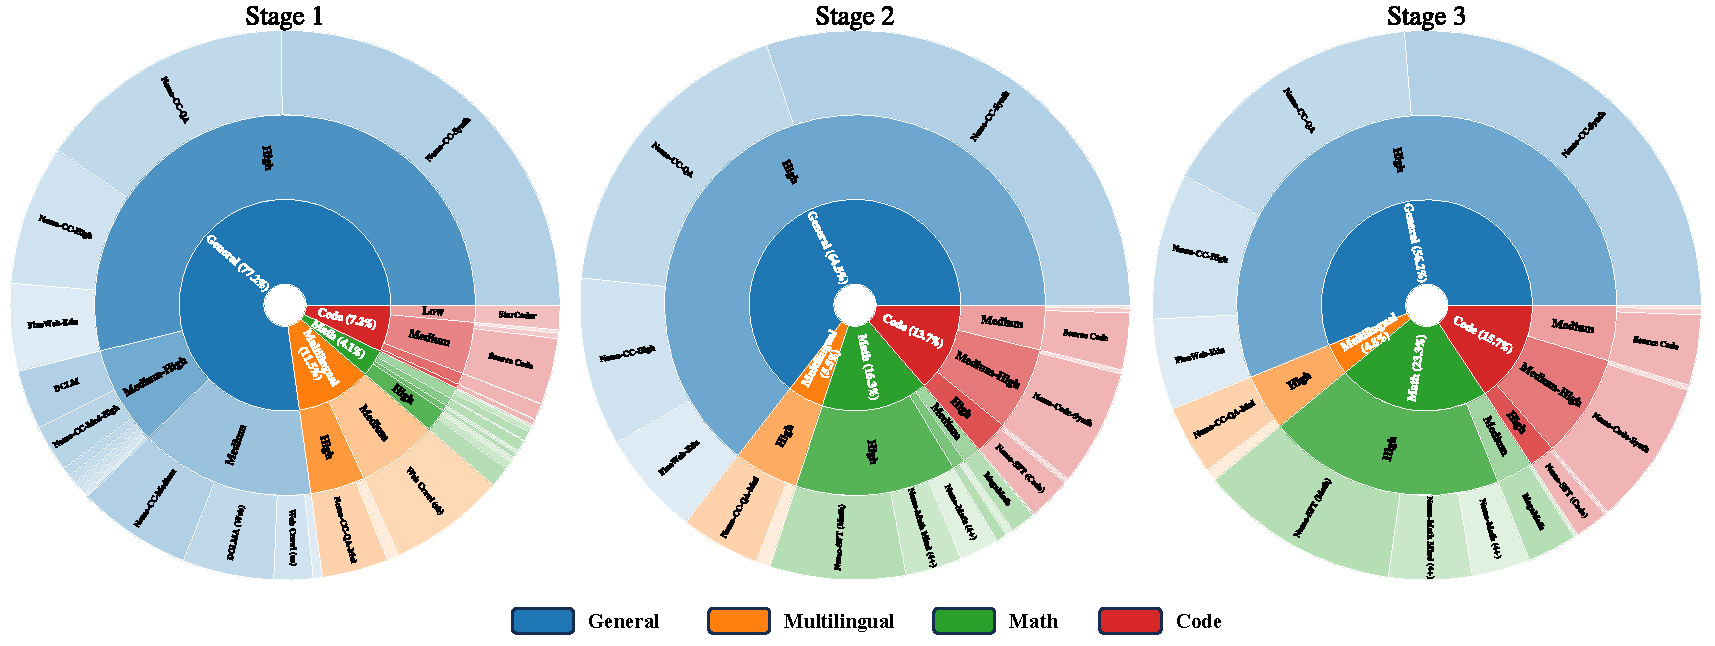
\includegraphics[width=.9\columnwidth]{fig/fig_dataset.pdf}}
    \caption{
      Data mixtures for the three stages of pre-training in the DeMix Corpora, with approximately 14T, 6T, and 2T tokens, respectively. The three hierarchical levels from the inside out are domain, data category, and data origin.
    }
      \label{fig:mixture_stages}
  \end{center}
\end{figure*}

\begin{table}[htbp]
\centering
\caption{Composition of DeMix Corpora and the mixture in each stage, measured in tokens (B).}
\label{table:dataset}
\resizebox{0.75\textwidth}{!}{% 如果表格过宽，可以使用 resizebox 缩放
\begin{tabular}{lllr|rrr}
\toprule
\textbf{Category} & \textbf{Quality} & \textbf{Original Source} & \textbf{Amount} & \textbf{Stage 1} & \textbf{Stage 2} & \textbf{Stage 3} \\
\midrule

% --- General (Total 15 rows) ---
\multirow{15}{*}{General} 
    & \multirow{4}{*}{High} 
      & FineWeb-Edu & 199 & 740 & 369 & 107 \\
    & & Nemo-CC-High & 385 & 1191 & 594 & 172 \\
    & & Nemo-CC-Synth & 1106 & 3630 & 1812 & 525 \\
    & & Nemo-CC-QA & 546 & 2190 & 1093 & 317 \\
    \cmidrule(lr){2-7}
    
    & \multirow{7}{*}{Medium-High} 
      & DCLM & 505 & 505 & 0 & 0\\
    & & DOLMA (Social) & 71 & 71 & 0 & 0\\
    & & Nemo-CC-Med-High & 393 & 393 & 0 & 0\\
    & & OpenCoder (Web) & 38 & 38 & 0 & 0\\
    & & Ultra-FineWeb (en) & 79 & 79 & 0 & 0\\
    & & DOLMA (Others) & 54 & 54 & 0 & 0\\
    & & Nemo-SFT (General) & 67 & 67 & 0 & 0\\
    \cmidrule(lr){2-7}
    
    & \multirow{4}{*}{Medium} 
      & DOLMA (Web) & 1278 & 774 & 0 & 0\\
    & & Web Crawl (en) & 1417 & 330 & 0 & 0\\
    & & Nemo-CC-Medium & 1605 & 965 & 0 & 0\\
    & & DOLMA (Scholar) & 77 & 77 & 0 & 0\\
\midrule

% --- Multilingual (Total 3 rows) ---
\multirow{3}{*}{Multilingual} 
    & \multirow{2}{*}{High} 
      & Ultra-FineWeb (zh) & 102 & 102 & 51 & 15 \\
    & & Nemo-CC-QA-Mul & 562 & 562 & 280 & 81 \\
    \cmidrule(lr){2-7}
    
    & Medium 
      & Web Crawl (zh) & 3304 & 991 & 0 & 0 \\
\midrule

% --- Math (Total 9 rows) ---
\multirow{9}{*}{Math} 
    & \multirow{3}{*}{High} 
      & Nemo-Math Mind (4+) & 69 & 69 & 199 & 98 \\
    & & Nemo-Math (4+) & 49 & 49 & 141 & 69 \\
    & & Nemo-SFT (Math) & 166 & 166 & 479 & 235 \\
    \cmidrule(lr){2-7}
    
    & Medium-High 
      & Reason (Math) & 38 & 38 & 36 & 0 \\
    & & SwallowMath & 31 & 31 & 29 & 0 \\
    \cmidrule(lr){2-7}
    
    & \multirow{2}{*}{Medium} 
      & MegaMath & 92 & 92 & 87 & 58 \\
    & & FineMath (4+) & 8 & 8 & 7 & 5 \\
    \cmidrule(lr){2-7}
    
    & \multirow{3}{*}{Low} 
      & Nemo-Math (3) & 76 & 76 & 0 & 0\\
    & & FineMath (3) & 20 & 20 & 0 & 0\\
    & & Math (Others) & 48 & 48 & 0 & 0\\
\midrule

% --- Code (Total 7 rows) ---
\multirow{7}{*}{Code} 
    & \multirow{2}{*}{High} 
      & Nemo-SFT (Code) & 45 & 45 & 150 & 39 \\
    & & OpenCoder & 6 & 6 & 20 & 5 \\
    \cmidrule(lr){2-7}
    
    & \multirow{3}{*}{Medium-High} 
      & Nemo-Code-Synth & 136 & 136 & 410 & 170 \\
    & & MegaMath (Code) & 5 & 5 & 15 & 6 \\
    \cmidrule(lr){2-7}
    
    & Medium 
      & Source Code & 559 & 559 & 200 & 83 \\
    & & SwallowCode & 47 & 47 & 17 & 7 \\
    & & Reason (Code) & 27 & 27 & 10 & 4 \\
    \cmidrule(lr){2-7}
    
    & Low 
      & StarCoder & 207 & 207 & 0 & 0 \\
\midrule
\multicolumn{3}{c}{\textbf{Total}} & \textbf{13417} & \textbf{14388} & \textbf{5999} & \textbf{1996} \\
      
\bottomrule
\end{tabular}
}
\end{table}




The data mixture used in LLM pre-training is inherently dynamic rather than static \cite{feng2024maximize, basant2025nvidia, blakeman2025nemotron}.
During the initial phases, the priority is typically given to data diversity, whereas the later stages shift focus toward high data quality \cite{wang2021survey}. 
In practice, early training stages typically emphasize data diversity, while late stages increasingly prioritize high-quality data to refine advanced capabilities \cite{wang2021survey}.
Consequently, pre-training is often organized into multiple stages, with the proportion of high-quality math and code data significantly increased in the late stages \cite{basant2025nvidia, allal2025smollm2}. 
As a result, modern pre-training pipelines are often organized into multiple stages, with the proportion of high-quality math and code data substantially increased in the late stages \cite{basant2025nvidia, allal2025smollm2}.

In practice, we partition the pre-training data into three stages, with the proportion of high-quality data such as mathematical and coding data gradually increasing across successive stages. In the first stage, as the model primarily acquires broad general knowledge during the initial phase of training, data quality exerts a less significant impact than in subsequent stages. Consequently, we only adjust the data mixture using basic general benchmarks, performing upsampling and downsampling based on quality scores. In contrast, during Stages 2 and 3, data quality directly influences the final training performance; thus, we employ the DeMix framework to optimize the data mixture ratio. Furthermore, to prevent excessive repetition of individual samples, we reduce the threshold for the allowable number of repetitions in Stage 2, yielding a more balanced data distribution compared to Stage 3.

We presents the detailed composition of DeMix Corpora in Figure \ref{fig:mixture_stages} and Table \ref{table:dataset}, including the amount of tokens after our curation pipeline and the token allocation in 3 training stages after data mixing by DeMix. 



\section{Baseline Details.}
\label{appd:train_detail}

For RegMix and CLIMB, the only differences from DeMix lie in how proxy models are obtained and how the predictor is trained.
For RegMix, we sample a required number of mixtures and train the model from the same initialization as the DeMix component models, using a fixed number of tokens. We then evaluate the trained models on to obtain benchmark scores, and fit a LightGBM predictor using the same hyperparameters as in DeMix. Finally, we apply the trained predictor to the same large set of sampled candidates and select the top-ranked mixtures as the final optimal mixture.
For CLIMB, the only difference is that it adopts iterative sampling. Consistent with our DeMix procedure, it performs three iterations: for 28 points, we sample $16+8+4$; for 56 points, $32+16+8$; for 112 points, $64+32+16$.



% \section{Delta of Model Parameters}

% \begin{figure*}[t]
%   \begin{center}
%     \centerline{\includegraphics[width=.8\columnwidth]{fig/heatmap.pdf}}
%     \caption{
%       Illustration of model $\delta$ between different checkpoints during component model training.
%     }
% \label{fig:heatmap}
%   \end{center}

% \end{figure*}

% As defined in Premise \ref{premise:small}, the delta of model parameters is given by $\delta=\frac{\sum|\mathcal{T}(D, \Theta_{\text{base}}) - \Theta_{\text{base}}|} {\sum|\mathcal{T}(D, \Theta_{\text{base}})| + \sum|\Theta_{\text{base}}|}$. A smaller $\delta$ indicates that the merged model is more stable and reliable. Figure \ref{fig:heatmap} shows that across our seven component models, $\delta$ is approximately 10\% with 30B tokens and 11\% with 50B tokens. These values reflect a relatively modest update magnitude. Therefore, our experiments generally operate within the Small Update Condition described in Premise \ref{premise:small}.

\section{Detailed Mixtures in Experiments.}
\label{appd:mixture}


\begin{table*}[!ht]
\caption{Detailed mixtures from different experiments.}
\label{table:mixture}
\centering
% \renewcommand{\arraystretch}{1.2} 
\setlength{\tabcolsep}{3.5pt}
\resizebox{0.8\textwidth}{!}
{
\begin{threeparttable}
\begin{tabular}{l|cccc|ccccccc}
\toprule

% --- 表头第一行 ---
\textbf{Method} & \multicolumn{4}{c}{\textbf{Train Cost (B) $\downarrow$}} & General & Math-1 & Math-2 & Math-3 & Code-1 & Code-2 & Code-3  \\

\midrule

% --- 数据部分 ---
Uniform & - & - & - & - & 0.500	&0.111	&0.027	&0.039	&0.020	&0.055	&0.248 \\
\midrule
Heuristic-2 & - & - & - & - & 0.400	&0.194	&0.024&	0.017	&0.052	&0.098	&0.216 \\
Heuristic-3 & - & - & - & - & 0.200	&0.273	&0.033&	0.000	&0.098	&0.136&	0.259 \\
\midrule

\multirow{3}{*}{\makecell[l]{RegMix} }
& 224 & - & 112 & 2 & 0.426	&0.336	&0.020	&0.012&	0.030&	0.074	&0.092 \\
& 224 & - & 28  & 8 & 0.710&	0.203&	0.003	&0.001	&0.079	&0.002	&0.002 \\
& 448 & - & 56  & 8 &  0.503	&0.330	&0.020&	0.001	&0.077	&0.009	&0.059 \\
\midrule
\multirow{3}{*}{\makecell[l]{CLIMB}} 
& 224 & - & 112 & 2 & 0.481	&0.366	&0.018&	0.008&	0.033&	0.034&	0.060 \\
& 224 & - & 28 & 8 & 0.714&	0.202&	0.002	&0.001&	0.078&	0.002&	0.002 \\
& 448 & - & 56 & 8 & 0.417	&0.422&	0.027&	0.011&	0.079&	0.008	&0.035  \\
\midrule
\multirow{4}{*}{\makecell[l]{DeMix\\(Ours)}} 
& 211 & 30$\times$7 & 56 & 0.01$\dagger$ & 0.017&	0.187	&0.406	&0.017	&0.135	&0.217	&0.022 \\
& 211  & 30$\times$7 & 112 & 0.01 & 0.271&	0.414&	0.009	&0.057	&0.046	&0.131	&0.073 \\
& 212  & 30$\times$7 & 224 & 0.01 & 0.218	&0.403	&0.002&	0.063	&0.044	&0.176	&0.094 \\
& 214 & 30$\times$7 & 448 & 0.01 & 0.454	&0.220&	0.006&	0.015	&0.077	&0.194	&0.034 \\
& 219  & 30$\times$7 & 896 & 0.01 & 0.181&	0.430&	0.004	&0.135	&0.029	&0.149&	0.071 \\
\bottomrule
\end{tabular}

\begin{tablenotes}
    \item $\dagger$ is the benchmarking cost derived from equal GPU‑hour as in Table \ref{table:cost}.
\end{tablenotes}
\end{threeparttable}
}
\end{table*}

We extend Table \ref{table:exp2} by listing the detailed mixture ratios in Table \ref{table:mixture}.

\section{Additional Verification of the Model-Merging Approximation}
\label{appd:merge_verification}

The approximation in Eq.~\ref{equ:satisfy} is mainly motivated by prior studies on model merging and small-update regimes. 
To further provide empirical evidence for its validity in our setting, we compare the merged proxy model with a model trained directly on mixed data. 
The goal is to verify whether the merged proxy model can consistently approximate the performance of the corresponding mixed-data-trained model, especially when the magnitude of parameter updates is relatively small.

Specifically, we select one math dataset as $D_1$ and one code dataset as $D_2$, and consider several mixture proportions between them. 
For each mixture proportion, we compare two types of proxy models:
\begin{itemize}
    \item \textbf{Model merge}: we first train two component models separately on $D_1$ and $D_2$, and then merge their parameters according to the target mixture ratio.
    \item \textbf{Data mix}: we directly train a model on the mixed dataset $D_1 + D_2$ with the same target mixture ratio.
\end{itemize}
We conduct this comparison under different token budgets. 
The parameter-update magnitude $\delta$ is computed as defined in Eq.~\ref{eqa:delta}. 
We define the consistency score as the ratio between the merged-model score and the data-mix model score on the same benchmark, averaged across all tested mixture proportions. 
A consistency score closer to $1$ indicates that the merged proxy model better matches the model trained directly on the corresponding mixed data.

The results are shown in Table~\ref{tab:merge_verification}. 
When $\delta$ is small, the merged proxy model exhibits high consistency with the data-mix model, suggesting that Eq.~\ref{equ:satisfy} is well satisfied in the small-update regime. 
As the token budget increases, $\delta$ naturally becomes larger, and the consistency moderately decreases. 
Nevertheless, even under relatively larger updates, the merged proxy model still preserves a reasonably high level of consistency, especially considering that it avoids training a separate model for every candidate mixture. 
These results provide additional empirical support for using merged proxy models to approximate mixed-data training during mixture search.

\begin{table*}[t]
\caption{
Comparison between merged proxy models and models trained directly on mixed data.
We use one math dataset $D_1$ and one code dataset $D_2$, and evaluate different $D_1/D_2$ mixture ratios.
$\delta$ denotes the magnitude of parameter updates as defined in Eq.~\ref{eqa:delta}.
Consistency is computed as the ratio between the merged-model score and the data-mix model score, averaged across the tested mixture ratios.
}
\centering
\small
\resizebox{\textwidth}{!}{
\begin{tabular}{c c c c c c c c c c c c c}
\toprule
\multirow{3}{*}{Token Budget} 
& \multirow{3}{*}{$\delta$}
& \multirow{3}{*}{Type}
& \multicolumn{8}{c}{$D_1/D_2$ Ratio}
& \multicolumn{2}{c}{} \\
\cmidrule(lr){4-11}
\cmidrule(lr){12-13}
& & 
& \multicolumn{2}{c}{20\%/80\%}
& \multicolumn{2}{c}{40\%/60\%}
& \multicolumn{2}{c}{60\%/40\%}
& \multicolumn{2}{c}{80\%/20\%}
& \multicolumn{2}{c}{Consistency} \\
\cmidrule(lr){4-5}
\cmidrule(lr){6-7}
\cmidrule(lr){8-9}
\cmidrule(lr){10-11}
\cmidrule(lr){12-13}
& & 
& Math & Code
& Math & Code
& Math & Code
& Math & Code
& Math & Code \\
\midrule

\multirow{2}{*}{2B} 
& \multirow{2}{*}{3.10\%}
& Model merge 
& 5.79 & 21.39 
& 6.26 & 20.09 
& 7.17 & 17.76 
& 8.38 & 15.94 
& \multirow{2}{*}{1.04} & \multirow{2}{*}{0.97} \\
& 
& Data mix 
& 6.03 & 21.56 
& 6.25 & 20.59 
& 6.64 & 18.16 
& 7.39 & 16.76 
& & \\

\midrule

\multirow{2}{*}{10B} 
& \multirow{2}{*}{6.90\%}
& Model merge 
& 6.49 & 25.12 
& 9.48 & 22.50 
& 11.55 & 18.05 
& 14.57 & 14.52 
& \multirow{2}{*}{0.96} & \multirow{2}{*}{0.81} \\
& 
& Data mix 
& 8.01 & 27.85 
& 9.28 & 23.31 
& 12.32 & 26.04 
& 13.66 & 20.99 
& & \\

\midrule

\multirow{2}{*}{30B} 
& \multirow{2}{*}{10.10\%}
& Model merge 
& 8.09 & 30.06 
& 11.17 & 23.09 
& 15.34 & 19.56 
& 19.95 & 15.42 
& \multirow{2}{*}{0.82} & \multirow{2}{*}{0.75} \\
& 
& Data mix 
& 11.79 & 30.87 
& 15.11 & 31.48 
& 18.26 & 29.45 
& 20.01 & 25.12 
& & \\

\midrule

\multirow{2}{*}{50B} 
& \multirow{2}{*}{10.50\%}
& Model merge 
& 8.48 & 33.19 
& 11.88 & 25.50 
& 15.74 & 20.97 
& 20.87 & 14.31 
& \multirow{2}{*}{0.79} & \multirow{2}{*}{0.75} \\
& 
& Data mix 
& 11.84 & 32.98 
& 17.36 & 33.10 
& 19.71 & 30.66 
& 22.11 & 27.44 
& & \\

\bottomrule
\end{tabular}
}
\label{tab:merge_verification}
\end{table*}
